\cotefile{109}
\scanpage{9}
\hfill\uline{Terminology}

\diagram{\small\begin{tabular}{@{}p{.72\linewidth}@{\quad}l@{}}
\inserted{primitive,} primary, secondary, ternary\ldots\ \unsure{structure} & 4.\\
standard type (iterated fibre products of) & 5.\\
$n$-stacks, $\infty$-stacks, \deleted{\unsure{an|en|n}} $n$-$\underline{C}$-stacks & 13.\\
Coherator & 13\\
Hot-equivalence of site \unsure{structure|structures} & 25\\
\hspace{1.5em}test category(!)\ \hrulefill & 26, \uline{39}\\
test-topology & 27\\
$\left.\begin{array}{@{}l@{}}
\text{modelizer !/ model-preserving}\quad\deleted{\unsure{41|4}}\\
\hfill\text{(or modelizing) functor !}
\end{array}\right\}$ &
\begin{minipage}{.22\linewidth}
\diagram{\begin{tikzcd}[ampersand replacement=\&,row sep=.1em,column sep=.55em]
{} \& \underline{41}\\
28 \arrow[ur] \arrow[dr] \& {}\\
{} \& \underline{42}
\end{tikzcd}}
\end{minipage}\\
$\left.\begin{array}{@{}l@{}}
\text{\unsure{'basic|basic} modelizer (Cat)}\\
\text{elementary modelizer(\unsure{!|;|!,})}
\end{array}\right)$ & $29^{\unsure{7|+}}$\\
\uline{Strict} \unsure{test.|test} category \deleted{\unsure{(!)|!|4.}} & 33, 39\\
standard simplices\quad\textemdash\ \textemdash\ \hrulefill & \\
\hspace{4em}cubes & 34\\
\begin{minipage}{.4\linewidth}
\figure{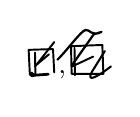
\begin{tikzpicture}[x=.26cm,y=.26cm,line cap=round,line join=round]
\draw[line width=.7pt] (0,0) -- (-.06,1.22) -- (1.13,1.26) -- (1.19,.12);
\draw[line width=1pt] (.06,.1) -- (.2,-.02) -- (.9,.03);
\draw[line width=.7pt] (.25,1.09) -- (.27,.04) .. controls (.19,-.12) and (-.02,-.08) .. (.07,.04);
\draw[line width=.7pt] (.25,.4) -- (1.19,1.6) (.25,.43) -- (.93,1);
\node at (1.58,-.01) {,};
\draw[line width=.7pt] (2.04,.05) -- (2.01,1.4) -- (3.54,1.46) -- (3.59,.05) -- cycle;
\draw[line width=.7pt] (2.18,1.32) -- (2.2,-.02) (2.04,.4) -- (3.09,.89);
\draw[line width=.8pt] (1.35,.74) .. controls (1.86,1.25) and (2.51,2.16) .. (2.72,2.19) .. controls (2.9,2.25) and (3.03,1.84) .. (3.5,2.1) -- (3.12,1.98) -- (2.05,.46);
\draw[line width=.75pt] (3.66,1.16) -- (3.02,.13) .. controls (2.77,-.37) and (3.22,-.15) .. (3.96,.41);
\end{tikzpicture}}
\end{minipage} & \deleted{34}\\
$\left.\begin{array}{@{}l@{}}
\text{aspheric (topos, object of topos, \inserted{map of objects})}\\
\text{locally \uline{aspheric topos, tot.\ asph.\ topos}}
\end{array}\right)$ & 35\\
\uline{Weak equivalence} ($f:X\mathrel{\unsure{-|\to}}Y$ \unsure{m}; of topos & ?\\
homotopy interval & 37\\
{}[strict] elementary modelizer & 39.\\
$\left.\begin{array}{@{}l@{}}
\text{local test \unsure{catégory|category}}\\
\text{local el.\ modelizer}
\end{array}\right)$ & 39\\
{}[locally] modelizing topos & 39
\end{tabular}}
% archive sheet number: 8

\scanpage{10}
\begin{center}Reflexions Mathématique\end{center}

(The simplest thing \inserted{for me} is to write out a\deleted{\unsure{n}} \inserted{possible} alternative version as our photocopy of the original is not that clear now. I'll underline in red places where the words are changed from your original whether by Breen or by us.)

After a twelve years' silence, the time has come for the author's works of maturity, with his vision and style renewed. Here is \uline{a} day-by-day account of an explorer's \deleted{travel} \inserted{\uline{journey}} with occasional reflections on the travel \uline{itself} \unsure{((|(}as well as on the traveler and the \uline{manifold} world around \uline{him},) \inserted{thus} recapturing its genuine nature: \uline{that} of an impassioned adventure, rooted in life

In the two forthcoming volumes, under the common title ``Pursuing Stacks'' (the first volume of which is subtitled ``The Modelizing Story,''), the author sketches some themes of a vast sythesis of homotopical algebra, (co)homological algebra and topos theory -- ripe now for more than fifteen years \uline{but} never yet begun. The leading thread, tenacious and omnipresent (while often remaining implicit) comes from algebraic geometry, and from the intuitions (rich precise and provocat\uline{ive}ly fragmentary) \uline{surrounding} the notions of sheaves, stacks, $2$-stacks ``etc.'' on a topos.

Thes two volumes are the first in a planned, considerably wider series of ``Réflexions Mathématiques'' \uline{in which} the author intends to \uline{present}, among other things, some ``naive ideas'' about two ``new continents'', eager to be discovered and explored. One \uline{stems from}
% archive sheet number: 9
\scanpage{11}
a suitable notion of a ``tame'' topological space, viewed as the natural set-up for expressing and stimulating the topological intuition of shape and form, which for so long has been squeezed \uline{into} the straitjacket of a ``General Topology'' tailored for the use of the analyst, not for geometry. This is inapt notably (because of pervasive ``wildness'' phenomena) for \uline{\inserted{the} study\deleted{ing} \inserted{of}} homotopy types of spaces of homeomorphisms, imbeddings \& the like, or for developing a \unsure{comprehensive} ``dévissage'' theory of stratified structures (whereas such structures \deleted{\unsure{abound}} \uline{crop up everywhere} notably in any question of ``moduli'' \deleted{\unsure{of}}for geometrical configurations capable of continuous variation and giving rise to degeneracy phenomena). The other continent appears \uline{at} the confluence of a multitude of streams of thought and insights, coming from topology, conformal geometry, algebraic geometry, discrete and profinite groups, algebraic groups over number fields, regular polyhedra, arithmetics, ``motives''\ldots, \uline{called together for} the exploration of the action of profinite ``absolute'' Galois groups (such as $\operatorname{Gal}_{\overline{\mathbb{Q}}/\mathbb{Q}}$) on certain (so called ``anabelian'') profinite geometrical fundamental groups (such as $\pi_{1}(P_{\overline{\mathbb{Q}}}-\{0,1,\infty\})$\unsure{,|.}

One of the leading threads comes from the combinatorial topology

(Continues without change until last paragraph)

The \inserted{two} first \deleted{two} volumes ``Pursuing Stacks'', started\unsure{\textendash|,} through the impetus of a correspondence in English are written in that language. They begin with a substantial common introduction \uline{of which a first part}, of personal rather than technical character, is written in French (the author's adopted language.).
% archive sheet number: 10

\scanpage{13}
\begin{center}\uline{COMMENTS ON ``PURSUING STACKS''}\end{center}

\diagram{\begin{tabular}{@{}l@{\quad}l@{}}
p2 $\ell$8 & inadequate\\
p2-$\ell$-15 & incomplete\\
p3 $\ell$-8 & pertinent\\
p4 $\ell$6 & indiscriminate\\
\hspace*{1.45em}$\ell$-1 & misled\\
p4-$\ell$-16 & arbitrary\\
\hspace*{1.45em}$\ell$-8 & the same\\
\multicolumn{2}{@{}l@{}}{Section 14 etc}\\
p2 $\ell$18 & impediment\\
p3 $\ell$4 & CW-spaces\\
\hspace*{1.45em}$\ell$12 & have\\
\hspace*{1.45em}$\ell$15 & adequate
\end{tabular}}

p3\qquad The question of cubical versus simplicial sets is an interesting one. The category of simplicial sets has a number of good properties, which have made it very popular.

1.\quad It is cartesian closed.

2.\quad The realisation functor gives an equivalence between the homotopy category of Kan simplicial sets and the homotopy category of CW-spaces and the proof of this has been published.

3.\quad The realisation functor satisfies $\lvert X\times Y\rvert$ is homeomorphic to $\lvert X\rvert\times\lvert Y\rvert$ (at least if one takes the fine topology with respect to compact subsets on the latter product, as is the correct thing to do for other purposes, such as obtaining the right cartesian closed category for topological spaces). Also simplicial sets are firmly embedded in the literature. Again, there is a Dold-Kan theorem, giving an equivalence between chain complexes and simplicial abelian groups. A neat proof of the Serre spectral sequence using simplicial methods has been published by A. Dress (see the reference in my paper with Heath ``Cogluing homotopy equivalences'').

By contrast, cubical sets are not greatly used in the literature, although a number of writers have found them convenient. A recent exposition by Massey of singular homology theory uses the cubical method throughout, and finds them very convenient. Again, Brown-Higgins have found them essential for their methods. The difficulties about using them are that they are not firmly embedded in the
% archive sheet number: 12
\scanpage{14}
\mspage{2}% typed -2-
literature. The proof of the equivalence of homotopy categories is not in the literature, indeed there is just this M.Phil. thesis of F. Hintze at Warwick which gives full details. (Part of the proof is also given by Federer in notes on algebraic topology from Brown University, 1962.) Cubical sets have a cartesian product, which does not have the correct realisation. This causes all sorts of difficulties. There is a tensor product which has the correct realisation, but having two products certainly complicates the issues. To obtain a Dold-Kan theorem, one has to introduce extra structure on cubical sets, namely the connections considered by Brown-Higgins. Realisations when you have this extra structure have not yet been worked out. More general notions of cubical groups, and related constructions, which have been well worked over by Kan and others in the simplicial case, have not yet been worked out for cubical groups.

$\ell$-3\qquad and \uline{a} corresponding.

p4 $\ell$8\qquad I would prefer here to talk about the Dold-Kan theorem, since Puppe only came in at a later stage, after the theorem had been proved independently by Dold and Kan. In fact Dold's original version was rather computational, and it was Kan who pointed out that the functor from chain complexes to simplicial abelian groups is given in a dimension $n$ by $\operatorname{Hom}(C_{N}\Delta^{n},C)$ for a chain complex $C$ . Also, a description of the theorem for a general additive category was done by Epstein.

It is curious that the way the Loday approach to homotopy type has gone is via $n$-simplicial sets although the proof of the modelling of all homotopy types is as yet incomplete. Similarly, the general van Kampen theory of Brown-Loday uses $n$-fold groupoids, more particularly $\mathrm{Cat}^{n}$-groups . I wonder whether the main problem is that to define gadgets like these for other situations, such as topoi, it may be necessary to have unit interval constructions, and this is where the various stack structures intervene, before obtaining the $\mathrm{Cat}^{n}$-groups.

$\ell$-7\qquad Replace eluding by evading.

$\ell$-2\qquad developed

p5 $\ell$8,9\quad Maybe it would be better as ``whereas it seems to me we have now come to a definite starting point''.

$\ell$11\qquad manifold

p7\qquad This construction of the nerve and its relation to homotopy types has been studied in detail by Fritsch and Latch.

p8\qquad The middle paragraph of this page is interesting. Certainly finding categories which model geometric situations, and then by the nerve obtaining a topological
% archive sheet number: 13
\scanpage{15}
\mspage{3}% typed -3-
space, has been found a very useful tool in geometric topology, particularly in recent work on the algebraic $K$-theory of topological spaces, by Waldhausen, and others. But it is fair to say that at this time it has not proved a \textit{basic} tool, and has not led itself to computation. An interesting test case is to try and determine $\pi_{3}(S^{2})$ without knowing about the Hopf fibration $S^{1}\to S^{3}\to S^{2}$ .

p9 $\ell$-5\qquad developing

p10 $\ell$6\qquad misled

$\ell$-15\quad standard. In many places, standart is used instead of standard.

p11 $\ell$10\quad the formal analogy

$\ell$12\qquad developing

$\ell$13\qquad standard

p12 $\ell$19\quad standard. Similarly lower down the page.

p13\qquad Isn't the reason that the category of all groupoids is not a topos is that it does not have a sub-object classifier?

p15 $\ell$18\quad Maybe omit ``still about''

p16 $\ell$11\quad ``This recalls to mind of course Quillen's''

$\ell$-5\qquad such a category

p17 $\ell$-2\quad commute with formation

\handwritten{so far, so good!}
% archive sheet number: 14

\scanpage{17}
\begin{center}Errors in 1\textsuperscript{st} 100 pages of notes + letter to Quillen.\end{center}

\uline{Quillen letter:}

``Commute with'' not ``commute to'' e.g p.5 line 14 - repeated.

Page 5 line 15 - ``including the structure of categories, groupoids\ldots.'' would be more normal.

Page $5'$, line 11, - ``standard'' not ``standar\deleted{d}t'' - repeated.

line -16, ``having \uline{the} same objects'' - article is missing

Page $6'$, line -13, ``each of the categor\uline{ies}''

\uline{Re}fl\uline{ections}

Page 1, line -13\quad ``indispensable''

2 line 18\quad ``impediments''

5 line 11\quad ``manifold'' - would be more usual

8 line - 8\quad ``adequate''

9 line 11\quad ``indispensable''

16 line 11\quad ``reminds'' needs an object eg. ``me'' or ``one''

21 line 12\quad ``$n$-tuples'' is I believe correct.

27 line -14\quad ``how can one define''

32 line 17 (middle of page) probably \unsure{`|``}modelizer''

34 line 6\quad ``which allow\ldots'' this phrase is not clear in sense.

``Allow'' with ``to'' usually takes an object i.e ``which allow one to\ldots'' but this doesn't seem to be right here

``Allow for'' is different.

39 line 18-``is'' not ``be''

41 line -6\quad ``we have'' is more correct than ``we got'' - which is American - $\therefore$ more like 16\textsuperscript{th} \unsure{or|+|\&} 17\textsuperscript{th} century English!
% archive sheet number: 16

\scanpage{18}
Page \deleted{\unsure{3|2}}41 \unsure{-}line -4\quad ``aspheric'' not ``asperic'' (avec\unsure{,|-} les asperges !\unsure{..|''})\unsure{..|.}

42, line -3, ``analogues'' would be more usual.

55 line 12, ``rather than just \uline{to} take $B$ and \uline{to} keep\ldots''

59 line -12, ``denote'' not ``debote''

60 line -11, ``of'' not ``ob''

61 line -20, ``Assume'' not ``Asumme''

63 line 16\quad ``make sense'' or ``have a sense''

66 line 13\quad I'm no \unsure{Latin|latin} expert but isn't it rather compositum (singular) composita (plural) than composita, compositae ? My Latin dictionary isn't \unsure{goodenough|good enough} to be sure !

p.77 line 12\quad ``isn't'' not ``is'nt'' this is repeated several times in different forms e.g ``does'nt'' for ``doesn't''

p.87 line 8\quad ``we \uline{have} only got to\ldots'' or ``we have only to\ldots''

p88 line 2\quad ``does'nt'' should be ``doesn't''; there is also an is'nt lurking around here.

p.89 line 3\quad ``to have got me'' or alternatively ``to have made me''

line 8\quad is ``very'' necessary?

line -15\quad \unsure{‘|``}last not least\unsure{’|''} is more usually ``last but not least''; an alternative would be ``last, not least,''.

P.90 line -15\quad ``compare'' takes ``with'' as does commute (4 occurences on this page)

line -9\quad some more ``is'nt''s .

line -8, replace ``,'' by ``that'' - this would give a better flow of words.
% archive sheet number: 17

\scanpage{19}
\mspage{2}% handwritten -2-

p.91 line 1. ``in view of\unsure{''|'} indicates a result of previous happenings

``with a view to'' indicates future hopes \& expectations

lines 15 \& 16 ``we've got'' or ``we have got'' is better.

line -16\unsure{.|,} ``avatars'' not ``avators''

p.92 line -16 probably ``informal'' is what you want (repeated in line -3)

p-99. $X$ and $Y$ have changed to $F$ \& $G$ it seems

p.100 line -16, ``having \uline{the} same objects''

% archive sheet number: 18

